\documentclass{article}

\usepackage{fontspec}
\usepackage{polyglossia}
\usepackage{notomath}
\setmainfont{GFS Artemisia}
\setsansfont{Source Code Pro}
\setmonofont{Source Code Pro}
\newfontfamily\greekfont[Script=Greek]{GFS Artemisia}
\newfontfamily\greekfontsf[Script=Greek]{GFS Artemisia}
\newfontfamily\greekfonttt[Script=Greek]{Source Code Pro}

%languages
\setdefaultlanguage{greek}
\setotherlanguages{english}


%typing
\usepackage{hyphenat}
\usepackage{float}
\usepackage{color, colortbl}
\usepackage{placeins}

%captions
\usepackage{caption}
\usepackage{subcaption}

%bib
% \usepackage{biblatex}
% \addbibresource{bib.bib}

%gemoetry
\usepackage[a4paper,top=1.2cm,bottom=1.2cm,left=1.2cm,right=1.2cm,marginparwidth=1.5cm]{geometry}

%images
\usepackage{graphicx}
\usepackage{tikz}

%ref
\usepackage[colorlinks=true, allcolors=blue]{hyperref}


\usepackage[export]{adjustbox}

%label
\usepackage{enumitem}
\renewcommand{\labelenumii}{\arabic{enumi}.\arabic{enumii}}
\renewcommand{\labelenumiii}{\arabic{enumi}.\arabic{enumii}.\arabic{enumiii}}
\renewcommand{\labelenumiv}{\arabic{enumi}.\arabic{enumii}.\arabic{enumiii}.\arabic{enumiv}}

%columnnew
\newcolumntype{g}{>{\columncolor{gray}}l}

%colors
\usepackage[dvipsnames]{xcolor}
\definecolor{gray}{gray}{0.9}
\definecolor{blue}{RGB}{82, 138, 174}
\definecolor{green}{RGB}{140, 219, 169}
\definecolor{yellow}{RGB}{253, 221, 92}

% \usepackage{titling}
% \setlength{\droptitle}{-20em}             %allagh glwssas
\hypersetup{
    colorlinks = true,
    linkcolor=black}


\usepackage{autobreak}


%Customize tables
\renewcommand{\arraystretch}{1.2}
% \rowcolors{2}{gray}{white}



\captionsetup[table]{
    format=plain,
    labelfont={small,it,bf}, % Small, italic, and bold label
    textfont={small,it}, % Italic text
    labelsep=colon % Colon separator
}



% Customize the figure caption
\captionsetup[figure]{
    format=plain,
    labelfont={small,it,bf}, % Small, italic, and bold label
    textfont={small,it}, % Italic text
    labelsep=colon % Colon separator
}

\makeatletter
\renewcommand*{\p@table}{\textit{Πίν. }}
\renewcommand*{\p@figure}{\textit{Σχ. }}
\renewcommand*{\p@equation}{\textit{Εξ. }}
\makeatother

\begin{document}
%TITLE
\newcommand{\uni}{ΑΡΙΣΤΟΤΕΛΕΙΟ ΠΑΝΕΠΙΣΤΗΜΙΟ ΘΕΣΣΑΛΟΝΙΚΗΣ}
\newcommand{\faculty}{ΠΟΛΥΤΕΧΝΙΚΗ ΣΧΟΛΗ}
\newcommand{\tmhma}{ΤΜΗΜΑ ΜΗΧΑΝΟΛΟΓΩΝ ΜΗΧΑΝΙΚΩΝ}


\newcommand{\titlos}{Δυναμικά φαινόμενα}
\newcommand{\ypotitlos}{Bonus Εργασία - Ειδικά Κεφάλαια Πεπερασμένων Στοιχείων}


\newcommand{\onomaauthor}{ΒΑΣΙΛΕΙΟΣ ΠΑΠΑΜΙΧΑΗΛ}


\newcommand{\advisor}{Γάκιας Χρήστος}
\newcommand{\mailauthor}{\href{mailto:vasilepi@meng.auth.gr}{vasilepi@meng.auth.gr}}
\newcommand{\aem}{6920}
\newcommand{\hmeromhnia}{\today}



\begin{titlepage}
    \begin{center}
    \raisebox{20mm}{
    \begin{tikzpicture}
        \draw (0,0) -- (6,0);
    \end{tikzpicture}}
\includegraphics[width=4cm]{media/autheng.jpg}\raisebox{20mm}{\begin{tikzpicture}
        \draw (0,0) -- (6,0);
    \end{tikzpicture}}
     \end{center}
    
    \begin{center}
        \large
        \uni\\
        \normalsize
        \faculty\\
        \vspace{1em}
        \tmhma
    \end{center}

    \vspace{2cm}
    \begin{center}
        \Large
        \textbf{\titlos}\\
        \vspace{1em}
        \large
        \textit{\ypotitlos}
    \end{center}
    \begin{center}
        \begin{tikzpicture}
        \draw (0,0) -- (4,0);
    \end{tikzpicture}\\
    \vspace{7em}
    \Large
    \textcolor{BrickRed}{\textbf{\onomaauthor}}\\
    \vspace{3em}
    
\includegraphics[width=0.3\textwidth]{media/newlogov3-cropped-content.png}
    \end{center}

    \vspace{7em}
    \hspace{4ex}
    \begin{minipage}[t]{0.45\textwidth} 
        \raggedright
        \textbf{Υπεύθυνος}: \advisor\\
        \textbf{Email}: \mailauthor\\
        \textbf{ΑΕΜ}: \aem
    \end{minipage}\\

    \vspace{4cm}
    \begin{center}
        \textit{\hmeromhnia}\\
        \begin{tikzpicture}
            \draw (0,0) -- (15,0);
        \end{tikzpicture}
    \end{center}
    
    
\end{titlepage}
\tableofcontents
%MAIN BODY


\section{Εισαγωγή}
\subsection{Παρουσίαση προβλήματος}

Στη παρόν εργασία ζητείται η ανάλυση ενός δυναμικού φαινομένου με τη χρήση Πεπερασμένων Στοιχείων. Πιο συγκεκριμένα, η επίλυση ενός προβλήματος ταλαντώσεων, με τη χρήση Explicit και Implicit μεθόδους για την εξακρίβωση της δυναμικής του συμπεριφοράς. Τα αποτελέσματα της επίλυσης συγκρίνονται με τα αναλυτικά για απλό πρόβλημα ταλαντώσεων.
\par Το πρόβλημα που επιλέχθηκε για επίλυση είναι το μοντέλο ενός μισού αυτοκινήτου υπό διέγερση εδάφους και στους δύο τροχούς. Το σασί του αυτοκινήτου μοντελοποιείται από στιβαρό σώμα του οποίου το κέντρο βάρους βρίσκεται σε απόσταση $L/3$ από τη μία άκρη. Το μήκος του σασί είναι $L = 4.5\; m$. Οι αναρτήσεις μοντελοποιούνται με μονοβάθμιους ταλανταντωτές με σημειακές μάζες, ενώ τα λάστιχα μοντελοποιούνται με σύστημα ελατηρίου-αποσβέστη. Το υπό επίλυση πρόβλημα φαίνεται στο \ref{fig:halfCar}.

\begin{figure}[H]
    \centering
    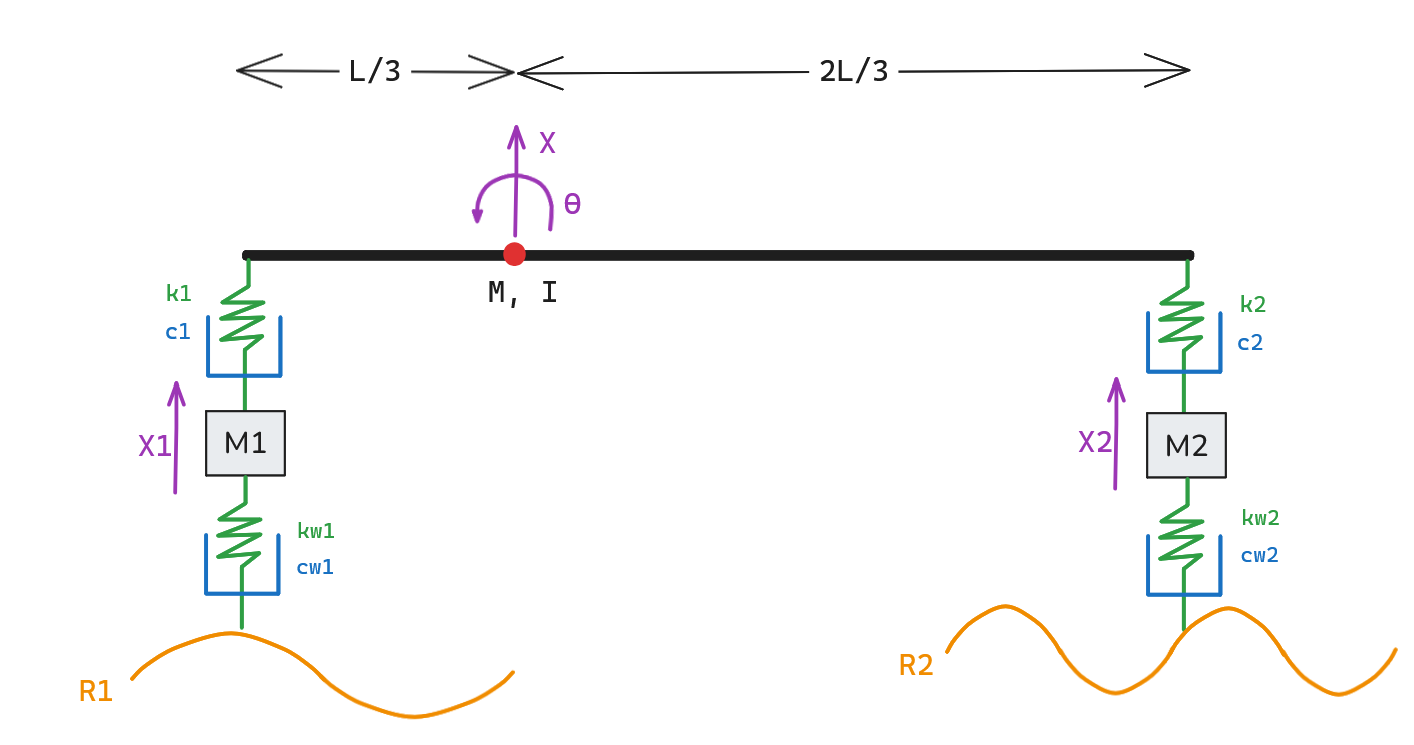
\includegraphics[width=0.8\linewidth]{media/halfCar.png}
    \caption{Σύστημα μισού αυτοκίνητου υπό διέγερση εδάφους.}
    \label{fig:halfCar}
\end{figure}

Οι σταθερές του προβλήματος φαίνονται παρακάτω στον \ref{tab:const}. Οι φορτίσεις της κατασκευής είναι ημιτονοειδείς σήματα με διαφορετικά πλάτη και συχνότητες. Ισχύει ότι:
\begin{equation}
\begin{aligned}
    r_1 &= R_1 \cdot sin(2\pi\Omega_1 \cdot t) \\
    r_2 &= R_2 \cdot sin(2\pi\Omega_2 \cdot t) 
\end{aligned}
\end{equation}

\begin{table}[H]
    \centering
    \rowcolors{2}{gray}{white}
    \begin{tabular}{|c|c|c|c|}
        \hline
        \rowcolor{Dandelion}
        Σταθερά & Τιμή & Σταθερά & Τιμή \\
        \hline
        $m$ & $1500\; kg$ & $c_{w1}$ & $150\; Ns/m$ \\
        \hline
        $I$ & $1805\; kg\,m^2$ & $c_{1}$ & $3000\; Ns/m$ \\
        \hline
        $m_1$ & $105\; kg$ & $c_{w2}$ & $160\; Ns/m$ \\
        \hline
        $m_2$ & $110\; kg$ & $c_{2}$ & $2800\; Ns/m$ \\
        \hline
        $k_{w1}$ & $360\times10^3\; N/m$ & $R_1$ & $0.1\; m$ \\
        \hline
        $k_{1}$ & $24.2\times10^3\; N/m$ & $R_2$ & $0.15\; m$ \\
        \hline
        $k_{w2}$ & $340\times10^3\; N/m$ & $\Omega_1$ & $10\; Hz$ \\
        \hline
        $k_{2}$ & $27.1\times10^3\; N/m$ & $\Omega_2$ & $15\; Hz$ \\
        \hline
    \end{tabular}
    \caption{Παράμετροι προβλήματος μισού αυτοκινήτου.}
    \label{tab:const}
\end{table}





\subsection{Αναλυτική επίλυση}
Το πρόβλημα έχει σύνολο 4 β.ε., μεταξύ αυτών 3 μεταφορικούς και έναν περιστροφικό. Επιλύοντας για κάθε β.ε. προκύπτουν οι εξισώσεις κίνησεις για κάθε σημειακή μάζα.

\begin{equation}
\begin{aligned}
    &m_1\ddot{x}_1 + (c_1 + c_{w1})\dot{x}_1 - c_1\dot{x} + c_1\frac{L}{3}\dot{\theta} + (k_1 + k_{w1})x_1 - k_1x + k_1\frac{L}{3}\theta = k_{w1}r_1 + c_{w1}\dot{r}_1 \\
    &m_2\ddot{x}_2 + (c_2 + c_{w2})\dot{x}_2 - c_2\dot{x} + 2c_2\frac{L}{3}\dot{\theta} + (k_2 + k_{w2})x_2 - k_2x + 2k_2\frac{L}{3}\theta = k_{w2}r_2 + c_{w2}\dot{r}_2 \\
    &m\ddot{x} - c_1\dot{x}_1 - c_2\dot{x}_2 + (c_1 + c_2)\dot{x} + \left(2c_2\frac{L}{3} - c_1\frac{L}{3}\right)\dot{\theta} - k_1x_1 - k_2x_2 + (k_1 + k_2)x + \left(2k_2\frac{L}{3} - k_1\frac{L}{3}\right)\theta = 0 \\
    &I\ddot{\theta} + c_1\frac{L}{3}\dot{x}_1 - 2c_2\frac{L}{3}\dot{x}_2 + \left(2c_2\frac{L}{3} - c_1\frac{L}{3}\right)\dot{x} + \left(c_1\frac{L^2}{9} + 4c_2\frac{L^2}{9}\right)\dot{\theta} \\
    &\quad + k_1\frac{L}{3}x_1 - 2k_2\frac{L}{3}x_2 + \left(2k_2\frac{L}{3} - k_1\frac{L}{3}\right)x + \left(k_1\frac{L^2}{9} + 4k_2\frac{L^2}{9}\right)\theta = 0
\end{aligned}
\end{equation}

Το παραπάνω σύστημα 4 εξισώσεων μπορεί να εκφραστεί και σε μητρωική μορφή εύκολα, με πίνακες:
$$
        M = \begin{bmatrix}
            m_1 & 0 & 0 & 0 \\
            
            0 & m_2 & 0 & 0 \\
            
            0 & 0 & m & 0 \\
            
            0 & 0 & 0 & I \\
        \end{bmatrix},\; C = \begin{bmatrix}
            c_1 + c_{w1} & 0 & -c_1 & \frac{c_1 L}{3} \\
            0 & c_2 + c_{w2} & -c_2 & -\frac{2 c_2 L}{3} \\
            -c_1 & -c_2 & c_1 + c_2 & \frac{(2 c_2 - c_1) L}{3} \\
            \frac{c_1 L}{3} & -\frac{2 c_2 L}{3} & \frac{(2 c_2 - c_1) L}{3} & \left( \frac{L}{3} \right)^2 (4 c_2 + c_1) \\        
        \end{bmatrix} 
$$
$$K = \begin{bmatrix}
            k_1 + k_{w1} & 0 & -k_1 & \frac{k_1 L}{3} \\
            0 & k_2 + k_{w2} & -k_2 & -\frac{2 k_2 L}{3} \\
            -k_1 & -k_2 & k_1 + k_2 & \frac{(2 k_2 - k_1) L}{3} \\
            \frac{k_1 L}{3} & -\frac{2 k_2 L}{3} & \frac{(2 k_2 - k_1) L}{3} & \left( \frac{L}{3} \right)^2 (4 k_2 + k_1) \\
\end{bmatrix},\; R = \begin{pmatrix}
    k_{w1}r_1 + c_{w1}\dot{r}_1\\
    k_{w2}r_2 + c_{w2}\dot{r}_2\\
    0\\
    0\\
\end{pmatrix}$$

Έτσι, μπορεί το σύστημα να μεταφραστεί σε μοντέλο state space με πίνακες:

$$
\mathbf{A}_N = 
\begin{bmatrix}
-\mathbf{M}^{-1} \mathbf{C} & -\mathbf{M}^{-1} \mathbf{K} \\
\mathbf{I} & \mathbf{0}
\end{bmatrix},\; \mathbf{B}_N = 
\begin{bmatrix}
-\mathbf{M}^{-1} \mathbf{L}_N \\
\mathbf{0}
\end{bmatrix}
$$

$$
\mathbf{C}_N = 
\begin{bmatrix}
-\mathbf{M}^{-1} \mathbf{C} & -\mathbf{M}^{-1} \mathbf{K} \\
\mathbf{I} & \mathbf{0} \\
\mathbf{0} & \mathbf{I}
\end{bmatrix}\;, \mathbf{D}_N = 
\begin{bmatrix}
\mathbf{M}^{-1} \mathbf{L}_N \\
\mathbf{0} \\
\mathbf{0}
\end{bmatrix}
$$

Όπου, $L_N$ ο πίνακας που εκφράζει το που εφαρμόζεται η φόρτιση και είναι:
$$L_N = \begin{bmatrix}
    1 & 0\\
    0 & 1\\
    0 & 0\\
    0 & 0\\
\end{bmatrix}$$

Τελικά, η επίλυση έγκειται στο state space σύστημα:
\begin{equation}
    \begin{aligned}
        \dot{z} &= A_N z + B_N R\\
        y &= C_N z + D_N R
    \end{aligned}
\end{equation}

Με τα διανύσματα μεταβλητής κατάστασης και εξόδου να είναι:

\begin{equation}
    z =\begin{bmatrix}
    x_1 & x_2 & x & \theta & \dot{x}_1 & \dot{x}_2 & \dot{x} & \dot{\theta}\\
\end{bmatrix}^T\\
\end{equation}


\begin{equation}
    y=\begin{bmatrix}
    z^T & \ddot{x}_1 & \ddot{x}_2 & \ddot{x} & \ddot{\theta}\\
\end{bmatrix}^T
\end{equation}


\section{Μονελοποίηση}
\subsection{Implicit}
Για την Implicit μοντελοποίηση, χρησιμοποιούνται στοιχεία MPC, SPRING, DASHPOT, MASS, ROTARYI. Το μοντέλο φαίνεται παρακάτω.
\begin{figure}[H]
    \centering
    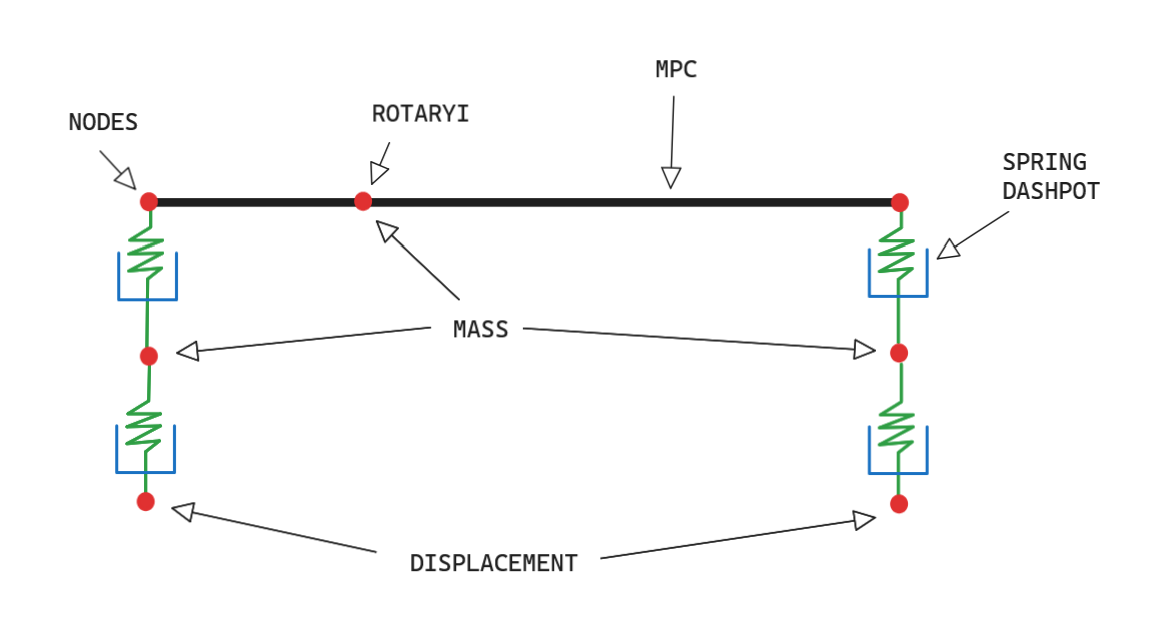
\includegraphics[width=0.6\linewidth]{media/imp.png}
    \caption{Μοντέλο Implicit επίλυσης.}
    \label{fig:imp}
\end{figure}

Στους κόμβους στο έδαφος, ορίζεται DISPLACEMENT με περιοδικό AMPLITUDE. Όσο αναφορά το STEP, συνολικός χρόνος επίλυσης ορίσθηκε Τ = 1 sec. και αριθμός βημάτων 5000 με βήμα επίλυσης 0.001 ώστε να καταγραφεί καλά η απόκριση από το ημιτονοειδείς σήμα.

\subsection{Explicit}
Για την Explicit μοντελοποίηση, πρέπει να δωθεί προσοχή στο γεγονός ότι ο ABAQUS/Explicit δεν υποστηρίζει στοιχεία SPTING, DASHPOT. Επομένως, για να προσομοιωθεί η συμπεριφορά του συστήματος ελατήριο-αποσβέστης, ορίζονται στοιχεία σύνδεσης τύπου CONN3D2. Για να λειτουργήσουν σωστά σαν ελατήρια, ο τύπος τους ορίζεται AXIAL. Έπειτα ορίζεται η συμπεριφορά στοιχείου σύνδεσης (CONNECTOR BEHAVIOR) ως ελαστικότητα και απόσβεση. Ενεργοποιείται το πρώτο COMPONENT της κάθε συμπεριφοράς ώστε να δρα στον άξονα X του τοπικού συστήματος αναφοράς του στοιχείου σύνδεσης, ο οποίος είναι στην διεύθυνση ορισμού του στοιχείου, δηλαδή στη διεύθυνση που δρα το ελατήριο και ο αποσβέστης. Να τονισθεί εδώ ότι για τον τύπο απόσβεσης δοκιμάστηκε τόσο η VISCOUS όσο και η STRUCTURAL. H VISCOUS προσέδιδε μεγάλη σταθερότητα στο μοντέλο κατά την επίλυση οποτέ είχε και πολύ καλύτερα αποτελέσματα. Με την STRUCTURAL απόσβεση, το σύστημα ήταν ασταθές και δε σύγκλινε. Παρακάτω φαίνεται το μοντέλο.
\begin{figure}[H]
    \centering
    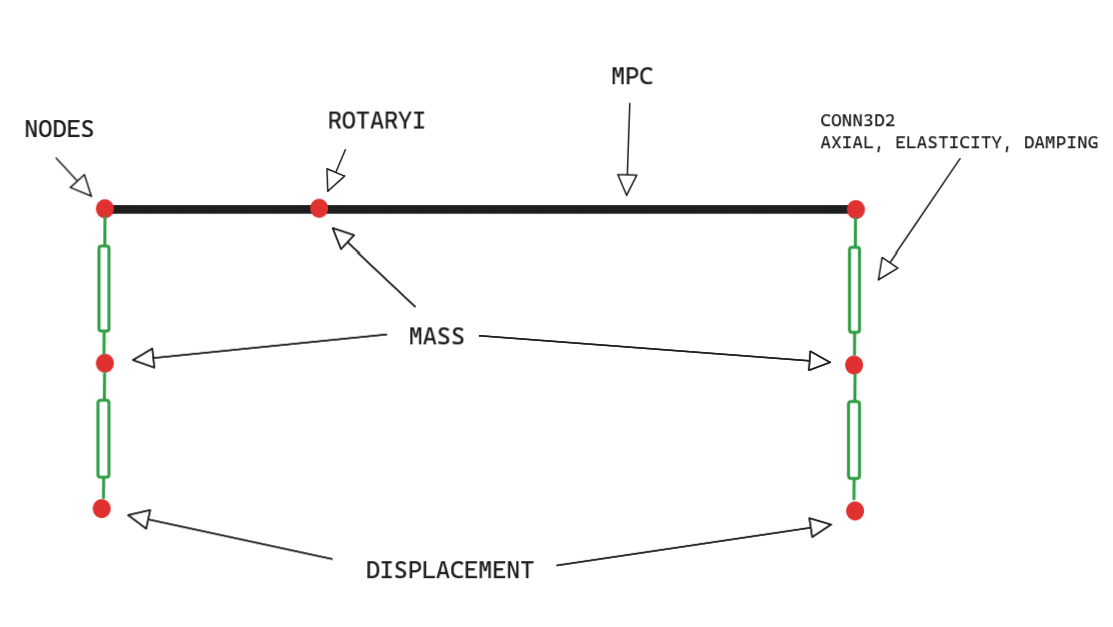
\includegraphics[width=0.6\linewidth]{media/exp.png}
    \caption{Μοντέλο Explicit επίλυσης.}
    \label{fig:exp}
\end{figure}

Για το STEP, ορίσθηκε INCREMENTATION σταθερό (DIRECT USER CONTROL) και ίσο με 1E-5 σύμφωνα με τις προδιαγραφές:
$$dt \le \frac{1}{100\cdot max\{\Omega_1,\Omega_2\}}$$

Να σημειωθεί ότι για την εξακρίβωση των δύο μοντέλων, έτρεξαν και αναλύσεις ιδιομορφικές (FREQUENCY) καθώς είναι εύκολες επιλύσεις. Αυτό έγινε για να συγκριθούν οι ιδιοτιμές των μοντέλων με τις αναλυτικές ώστε να αποδειχθεί ότι τα στοιχεία μοντελοποίησης προσομοιώνουν καλά τη κατασκευή. Οι ιδιομορφικές αναλύσεις επιλύθηκαν με LANCZOS για τις 4 πρώτες ιδιοτιμές από 0.01 - 2000 Hz.

\section{Αποτελέσματα Και Συζήτηση}
\subsection{Αποτελέσματα}

Παρακάτω φαίνονται οι συγκρίσεις της αναλυτικής επίλυσης με τις δύο προσεγγίσεις πεπερασμένων στοιχείων.

\begin{figure}[H]
    \centering
    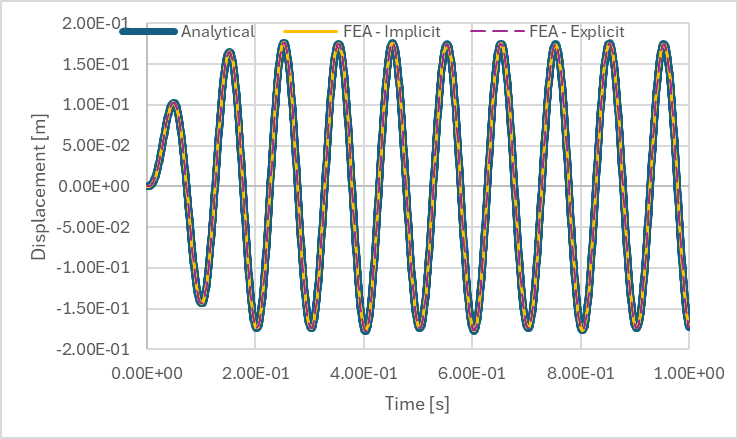
\includegraphics[width=0.8\linewidth]{media/d-x1.png}
    \caption{Απόκριση μετατόπισης οπίσθιας ανάρτησης αυτοκινήτου $x_1$, σε αρμονική διέγερση εδάφους.}
    \label{fig:d-x1}
\end{figure}

\begin{figure}[H]
    \centering
    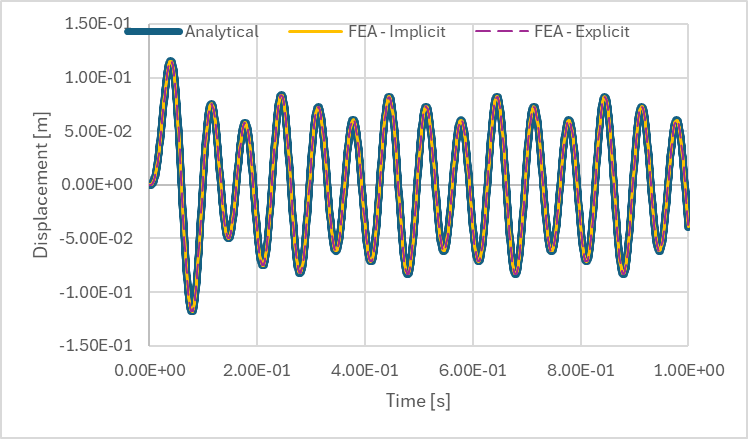
\includegraphics[width=0.8\linewidth]{media/d-x2.png}
    \caption{Απόκριση μετατόπισης εμπρόσθιας ανάρτησης αυτοκινήτου $x_2$, σε αρμονική διέγερση εδάφους.}
    \label{fig:d-x2}
\end{figure}

\begin{figure}[H]
    \centering
    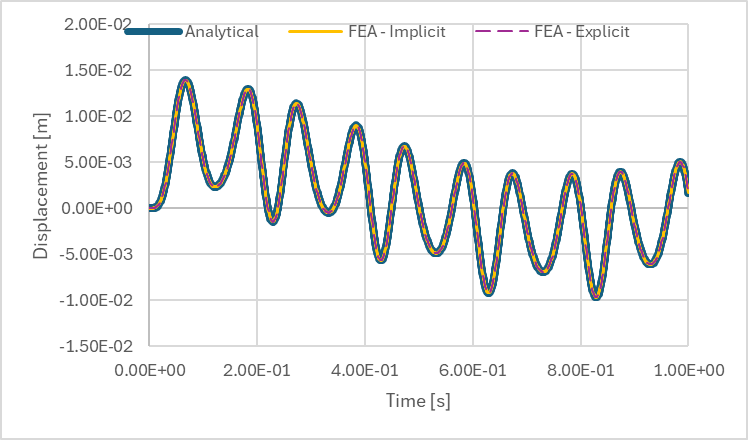
\includegraphics[width=0.8\linewidth]{media/d-x.png}
    \caption{Απόκριση μετατόπισης σασί αυτοκινήτου $x$, σε αρμονική διέγερση εδάφους.}
    \label{fig:d-x}
\end{figure}

\begin{figure}[H]
    \centering
    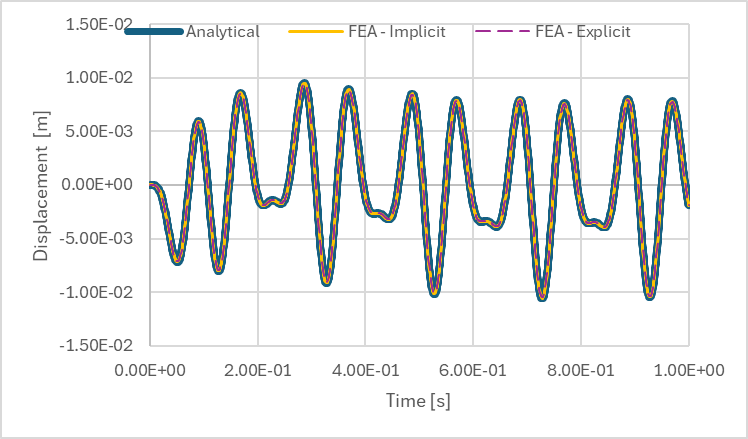
\includegraphics[width=0.8\linewidth]{media/d-th.png}
    \caption{Απόκριση περιστροφής σασί αυτοκινήτου $\theta$ σε αρμονική διέγερση εδάφους.}
    \label{fig:d-th}
\end{figure}

Πέρα από τις μετατοπίσεις των βαθμών ελευθερίας, διαβάζονται επίσης και οι επιταχύνσεις του σασί του αυτοκινήτου. Παρακάτω φαίνονται τα αποτελέσματα για τους βαθμούς ελευθερίας της μάζας $m$ στο πεδίο του χρόνου.

\begin{figure}[H]
    \centering
    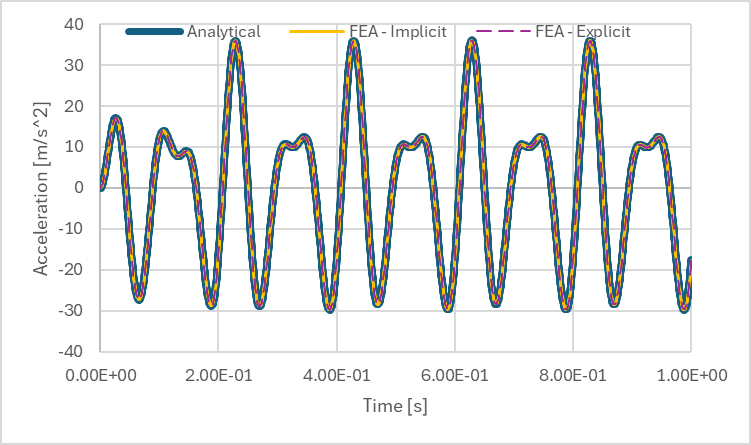
\includegraphics[width=0.8\linewidth]{media/a-x.png}
    \caption{Απόκριση μεταφορικής επιτάχυνσης σασί αυτοκινήτου $\ddot{x}$ σε αρμονική διέγερση εδάφους.}
    \label{fig:a-x}
\end{figure}

\begin{figure}[H]
    \centering
    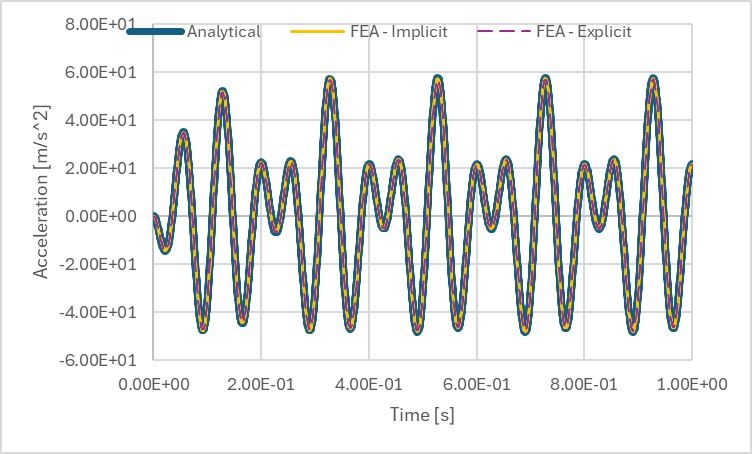
\includegraphics[width=0.8\linewidth]{media/a-th.png}
    \caption{Απόκριση περιστροφικής επιτάχυνσης σασί αυτοκινήτου $\ddot{\theta}$ σε αρμονική διέγερση εδάφους.}
    \label{fig:a-th}
\end{figure}

\subsection{Συζήτηση}
Όπως φαίνεται, παρατηρείται πλήρη ταύτιση των αποτελέσματων με την αναλυτική επίλυση. Αυτό δείχνει ότι για το απλό πρόβλημα δυναμικής απόκρισης, μισού αυτοκινήτου, υπό αρμονική διέγερση εδάφους, και οι δύο προσεγγίσεις (Implicit, Explicit) ανταποκρίνονται πολύ καλά. Ωστόσο, η επίλυση με Explicit μεθόδους, ήταν πολύ πιο ασταθής και χρειάστηκε να καταβληθεί πολύ μεγαλύτερη προσπάθεια για να σταθεροποιηθεί η επίλυση. Χρειάστηκε να εξετασθούν πολύ πιο ενδελεχώς οι παράμετροι της επίλυσης και να δωθεί πολύ μεγαλύτερη βάση στη μοντελοποίηση. Μια μικρή παράμετρος όπως ο τύπος απόσβεσης επηρέαζε δραματικά την απόκριση από εντελώς ασταθή σε ταυτόσιμη με την αναλυτική επίλυση. Επομένως, καταλήγει κανείς, ότι για τόσο απλό πρόβλημα όσο αυτό της συγκεκριμένης εργασίας, η Implicit επίλυση αποτελεί καλύτερη επιλογή λόγω της ευκολίας χρήσης του ABAQUS/Standard. Μπορεί η Explicit επίλυση να ήταν πιο γρήγορη στο να επιφέρει αποτελέσματα αλλά ήταν πολύ πιο χρονοβόρα στο να βρεθούν οι κατάλληλες παράμετροι που σταθεροποιούν την επίλυση.













\listoffigures
\listoftables

\end{document}